\chapter{Elaboration of the Workflow}
\label{chap:elaboration-of-the-workflow}

In this chapter I demonstrate the various steps of the workflow in detail. I introduce small working source code examples and show, how the given step transforms it.

\section{Transforming the Source Code Into an AST}
As mentioned in~\Cref{sect:overview-transforming-the-source-code}, this transformation is carried out by the Shape Security Shift toolkit. The parser is given the source code and the top-level non-terminal it should consider the root of the tree. Considering the new constructs introduced in ES6, I've chosen \emph{Module} as the type of the root.

The only one line long source code in~\Cref{lst:oneliner} parsed and serialized as a tree can be seen in~\Cref{lst:oneliner-ast-json}.

\begin{figure}[!ht]
	\begin{minipage}{\textwidth}
		\lstinputlisting[captionpos=b,caption={Basic example source code.},label={lst:oneliner},commentstyle=\color{black},language=JavaScript]{include/sources/oneliner.js}
	\end{minipage}
\end{figure}

\begin{figure}[!ht]
	\begin{minipage}{\textwidth}
		\lstinputlisting[captionpos=b,caption={AST output of the parser serialized in JSON format.},label={lst:oneliner-ast-json},commentstyle=\color{black},language=JSON]{include/sources/oneliner-ast.json}
	\end{minipage}
\end{figure}

\section{Storing the ASG in the Graph Database}

\section{Division by Zero}
As one of the most basic and easy-to-discover mistakes, division by zero should be reported to the developer. In the context of mathematics, division by zero is undefined for the real numbers. In JavaScript, it may result in \code{NaN} or \code{Infinity}.

Without dynamic testing or symbolic execution it is rather hard to find this kind of expression, since the right side of the division may come from a variable. On the other hand, finding the cases where the right side is a literal is trivial.

Taking a look at the graph representation of the previous example (in~\Cref{fig:AST-PPT}), it is relatively easy to find the problematic nodes. A natural language definition of the problem would sound like: ,,we are looking for binary expressions that have a literal zero on the right side''.

\begin{figure}[!htb]
  \centering
  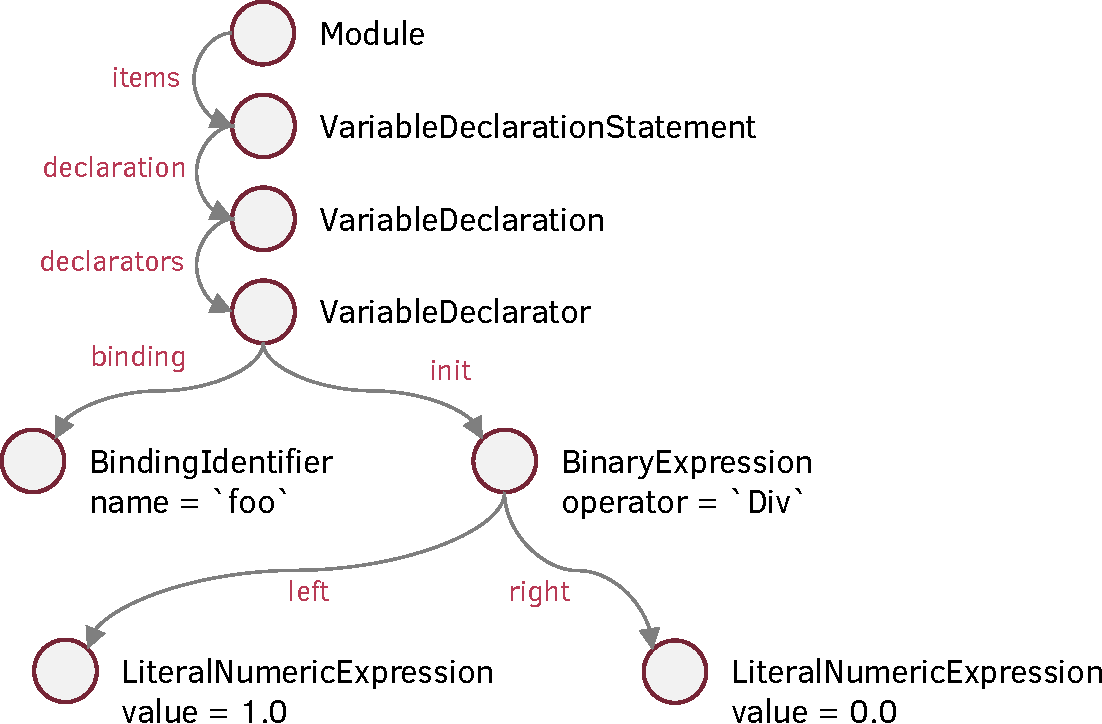
\includegraphics[width=0.5\textwidth]{AST-PPT.pdf}
  \caption{Graph Representation of the One Line Long Source Code}
  \label{fig:AST-PPT}
\end{figure}

One way to formalize this declarative definition in Cypher can be seen in~\Cref{lst:division-by-zero}. Executing this query would find matching nodes with the right type, bind them to the corresponding names and check, whether the required relations are present, resulting in a state like in~\Cref{fig:AST-query-PPT}. Finally the result is the \code{BinaryExpression} node that can be used to get the precise location of the expression in the source code and report it as problematic.

\begin{figure}[!ht]
	\begin{minipage}{\textwidth}
		\lstinputlisting[captionpos=b,caption={Graph Pattern Matching Division by Zero.},label={lst:division-by-zero},language=Cypher]{include/sources/division-by-zero.cypher}
	\end{minipage}
\end{figure}

\begin{figure}[!htb]
  \centering
  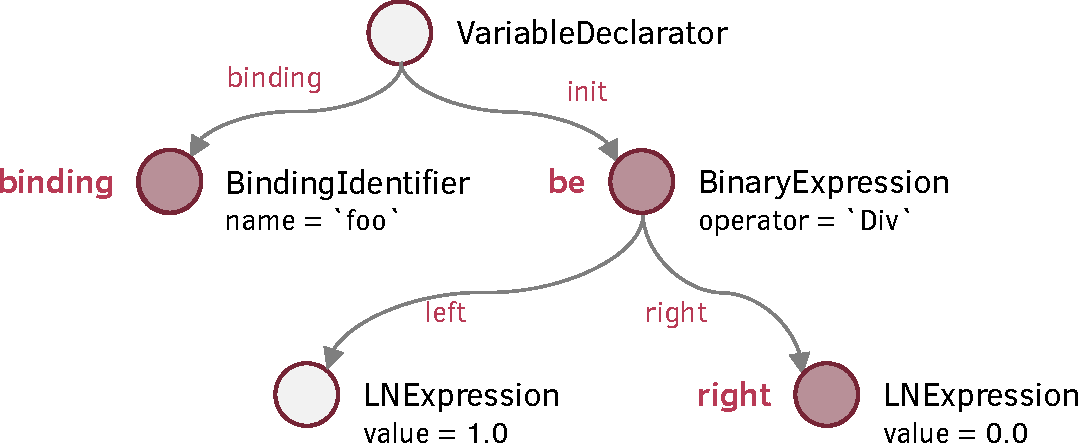
\includegraphics[width=0.5\textwidth]{AST-query-PPT.pdf}
  \caption{Graph Representation of the Query Searching Division by Zero}
  \label{fig:AST-query-PPT}
\end{figure}

\section{Dead Code Search}

\section{Control Flow Graph}

\section{Language Limitations}
